%!TEX TS-program = lualatex
%!TEX encoding = UTF-8 Unicode
\documentclass[a4paper, 11pt, parskip=half]{scrartcl}

% ============================================================
% PRÄAMBEL & PAKETE (Design Herr Dayi)
% ============================================================
\usepackage[a4paper, top=1.6cm, bottom=1.8cm, left=2.0cm, right=1.8cm, footskip=0.8cm]{geometry}
\usepackage[ngerman]{babel}
\usepackage{fontspec}
\setmainfont{Libertinus Serif}
\setsansfont{Latin Modern Sans}
\usepackage{amsmath, amssymb}
\usepackage{multicol} 
\usepackage{lineno} 
\usepackage{changepage} 
\usepackage{enumitem} 
\usepackage{graphicx} 
\usepackage{qrcode}
\usepackage{xcolor}
\usepackage[most]{tcolorbox}
\usepackage{tabularx}
\usepackage{tikz}

\definecolor{primaryBlue}{RGB}{20, 50, 100} 
\definecolor{lightBlue}{RGB}{245, 248, 253}
\definecolor{accentBlue}{RGB}{37, 99, 235}

% --- Sozialform-Piktogramme ---
\newcommand{\tikzUser}[1]{%
    \begin{tikzpicture}[x=0.07cm,y=0.07cm, baseline=-0.8ex]
        \fill[#1] (0,3.5) circle (1.5);
        \fill[#1] (-2,0) .. controls (-2,1.5) and (-1.5,2) .. (0,2) .. controls (1.5,2) and (2,1.5) .. (2,0) -- (-2,0) -- cycle;
    \end{tikzpicture}%
}
\newcommand{\iconEA}{\begin{tikzpicture}[baseline=(char.base)]\node[draw=primaryBlue, thin, inner sep=2pt, fill=white] (char) {\tikzUser{primaryBlue} \scalebox{0.6}{EA}};\end{tikzpicture}}
\newcommand{\iconPA}{\begin{tikzpicture}[baseline=(char.base)]\node[draw=primaryBlue, thin, inner sep=2pt, fill=white] (char) {\tikzUser{primaryBlue}\hspace{-1pt}\tikzUser{primaryBlue} \scalebox{0.6}{PA}};\end{tikzpicture}}
\newcommand{\iconGA}{\begin{tikzpicture}[baseline=(char.base)]\node[draw=primaryBlue, thin, inner sep=2pt, fill=white] (char) {\tikzUser{primaryBlue}\hspace{-1pt}\tikzUser{primaryBlue}\hspace{-1pt}\tikzUser{primaryBlue} \scalebox{0.6}{GA}};\end{tikzpicture}}

% Aufgaben-Umgebung
\newcounter{aufgabencnt}
\newenvironment{aufgabe}[1]{ 
    \stepcounter{aufgabencnt}
    \vspace{0.25cm}
    \noindent\begin{tikzpicture}[baseline=(char.base)]
        \node[draw=primaryBlue, fill=primaryBlue, text=white, font=\small\bfseries, inner sep=3pt] (char) {Aufgabe \arabic{aufgabencnt}};
    \end{tikzpicture} \hspace{0.1cm} \hfill #1\par\medskip
}{%
    \par\vspace{0.15cm}
}

\newcommand{\runningMan}{%
\begin{tikzpicture}[scale=0.18, baseline=-1mm, thick]
    \draw (0,1) circle (0.4); 
    \draw (0,0.6) -- (0,-0.2); 
    \draw (0,0.4) -- (-0.6,0); 
    \draw (0,0.4) -- (0.6,0.8); 
    \draw (0,-0.2) -- (-0.5,-0.8); 
    \draw (0,-0.2) -- (0.5,0); \draw (0.5,0) -- (0.8,-0.8); 
\end{tikzpicture}}

\modulolinenumbers[5] 
\setlength\linenumbersep{10pt} 
\renewcommand\linenumberfont{\normalfont\tiny\sffamily\color{gray}}

\begin{document}

% ================= SEITE 1: TEXT UND INFOKASTEN =================

\noindent
\begin{minipage}[t]{0.48\textwidth}\textbf{Philosophie Q1} \\ Herr Dayi\end{minipage}%
\hfill
\begin{minipage}[t]{0.48\textwidth}\raggedleft Datum: \rule{2.5cm}{0.4pt}\end{minipage}

\vspace{0.15cm}
\hrule height 0.8pt
\vspace{0.35cm}

% --- QR-CODE MIT HILFESTELLUNG ---
\marginpar{\vspace{0.05cm}\hspace{-2.2cm}\centering%
\qrcode[height=1.2cm]{https://herrdayi.github.io/Freud/}\\[0.15cm]%
{\tiny\sffamily\color{primaryBlue}\hspace{-2.2cm}\textbf{Hilfe}}}

\noindent {\Large \textbf{\color{primaryBlue}Sigmund Freud – Das Unbehagen in der Kultur (1930)}}
\vspace{0.35cm}

% === TEXTBEREICH MIT RECHTEM NOTIZRAND & STRUKTURIERTEN ABSCHNITTEN ===
\begin{adjustwidth}{0cm}{1.8cm}
\normalsize\linespread{1.12}\selectfont
\begin{linenumbers}

\noindent „Der Mensch ist eben nicht ein sanftes, liebebedürftiges Wesen, das sich höchstens, wenn 
angegriffen, zu erwehren vermag, sondern er darf unter seinen Triebbegabungen auch einen 
mächtigen Anteil von Aggressionsneigung rechnen. Infolgedessen ist ihm der Nächste nicht nur 
möglicher Helfer und Sexualobjekt, sondern auch eine Versuchung, seine Aggression an ihm zu 
befriedigen, seine Arbeitskraft ohne Entschädigung auszunützen, ihn ohne seine Einwilligung 
sexuell zu gebrauchen, sich in den Besitz seiner Habe zu setzen, ihn zu demütigen, ihm 
Schmerzen zu bereiten, ihn zu martern und zu töten. \textit{Homo homini lupus}; wer hat nach allen 
Erfahrungen des Lebens und der Geschichte den Mut, diesen Satz zu bestreiten? [\dots] Das 
Dasein dieser Aggressionsneigung [\dots] stört unser Verhältnis zum Nächsten und nötigt die 
Kultur zu ihrem Aufwand. Infolge dieser primären Feindseligkeit der Menschen gegeneinander 
ist die Kulturgesellschaft beständig vom Zerfall bedroht.“

\vspace{0.4cm}
\noindent „Die Kultur muss alles aufbieten, um den Aggressionstrieben der Menschen Schranken zu 
setzen, ihre Äußerungen durch psychische Reaktionsbildungen niederzuhalten. Daher also das 
Aufgebot von Methoden, welche die Menschen zu Identifizierungen und zielgehemmten 
Liebesbeziehungen antreiben sollen, daher die Einschränkung des Sexuallebens und daher 
auch das Idealgebot, den Nächsten so zu lieben wie sich selbst, das sich ja wirklich 
dadurch rechtfertigt, dass nichts anderes der ursprünglichen Menschennatur so sehr 
widerspricht. [\dots] Der Kulturmensch hat für ein Stück Glücksmöglichkeit ein Stück 
Sicherheit eingetauscht. [\dots] Das Zusammenleben der Menschen wird eben erst ermöglicht, 
wenn sich eine Mehrheit zusammenfindet, die stärker ist als jeder Einzelne und gegen 
jeden Einzelnen zusammenhält.“

\vspace{0.4cm}
\noindent „Was geschieht im Individuum, um seine Aggressionslust unschädlich zu machen? [\dots] Die 
Aggression wird introjeziert, verinnerlicht, sie wird eigentlich dorthin zurückgeschickt, 
woher sie gekommen ist, also gegen das eigene Ich gewendet. Dort wird sie von einem 
Teil des Ichs übernommen, der sich als Über-Ich dem übrigen gegenüberstellt, und nun als 
»Gewissen« gegen das Ich dieselbe strenge Aggressionsbereitschaft ausübt, die das Ich 
gerne an anderen, fremden Individuen befriedigt hätte. Die Spannung zwischen dem 
strengen Über-Ich und dem ihm unterworfenen Ich heißen wir Schuldbewusstsein; es 
äußert sich als Strafbedürfnis. Die Kultur bezwingt also die gefährliche Aggressionslust 
des Individuums, indem sie es schwächt, entwaffnet und durch eine Instanz in seinem 
Innern, wie durch eine Besatzung in der eroberten Stadt, überwachen lässt.“

\end{linenumbers}
\vspace{0.15cm}
\tiny {
(Zusammengestellt nach den Originalfassungen in: Sigmund Freud: \textit{Das Unbehagen in der Kultur} [1930], Kapitel V und VII. In: Gesammelte Werke, Band XIV, Frankfurt am Main: Fischer 1999.)}
\end{adjustwidth}

\vspace{\fill}

% === INFOKASTEN MIT HISTORISCH-PHILOSOPHISCHEM KONTEXT ===
\begin{tcolorbox}[
    enhanced, colback=lightBlue, colframe=primaryBlue, boxrule=0.8pt, arc=0mm,
    title=\textbf{Zur Person: Sigmund Freud (1856–1939)}, fonttitle=\small\bfseries\color{white},
    attach boxed title to top left={yshift=-2mm, xshift=2mm},
    boxed title style={colback=primaryBlue, arc=0mm, boxrule=0pt},
    boxsep=4pt, bottom=4pt, top=6pt
]
\footnotesize
\begin{tabularx}{\textwidth}{X r}
Sigmund Freud war ein österreichischer Arzt, Neurophysiologe und der Begründer der modernen \textit{Psychoanalyse}. Tief geprägt von den Erfahrungen des Ersten Weltkriegs und den gesellschaftlichen Krisen seiner Zeit wandte er sich in seinen späten Schriften zunehmend kulturphilosophischen Fragen zu. In seinem Werk \textit{Das Unbehagen in der Kultur} (1930) untersucht er das spannungsgeladene Verhältnis zwischen den biologischen Antrieben des Menschen und den Anforderungen des zivilisierten Zusammenlebens -- und geht der Frage nach, warum menschliche Kultur stets von einer inneren Zerbrechlichkeit bedroht bleibt. & 
\raisebox{-0.85\height}{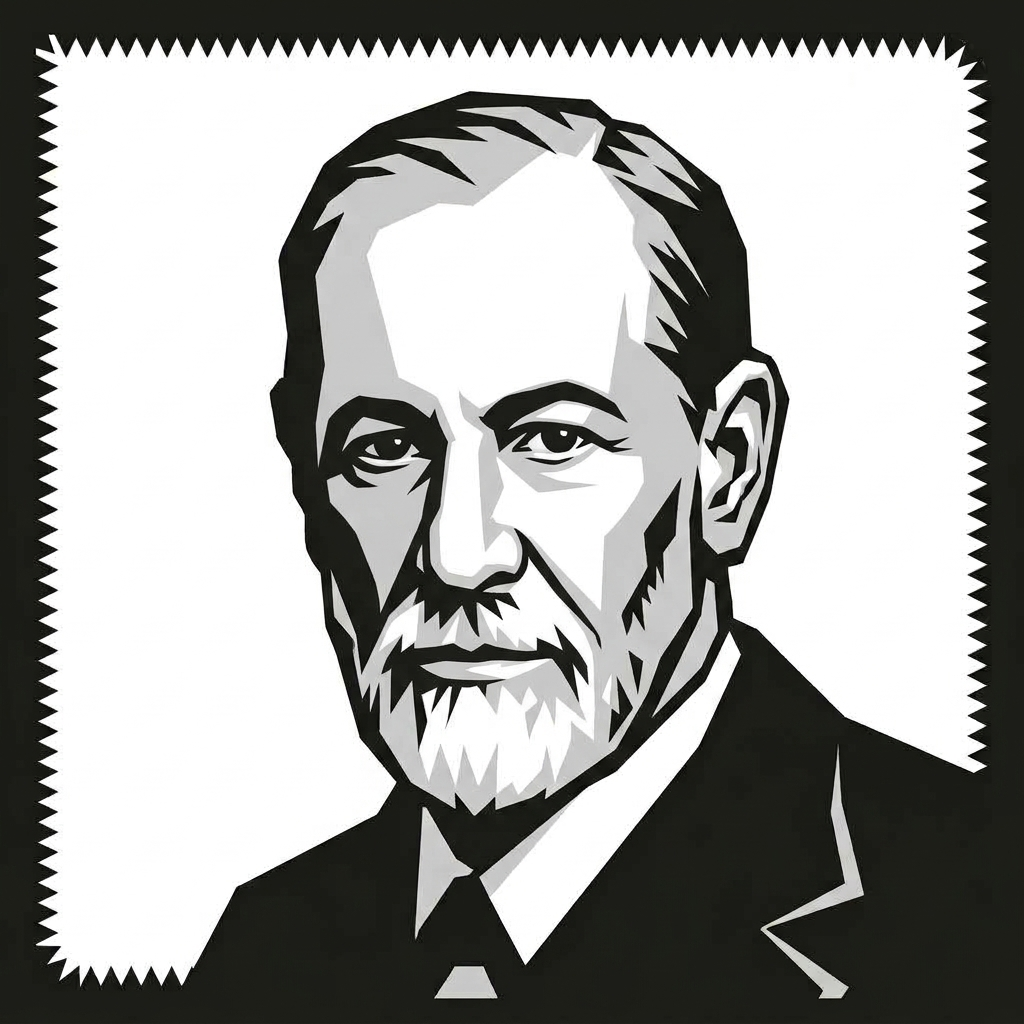
\includegraphics[width=2.1cm]{Freud.png}} 
\end{tabularx}
\end{tcolorbox}

\newpage % ================= SEITE 2: ARBEITSAUFTRÄGE & METHODENKARTE =================

\noindent {\Large \textbf{\color{primaryBlue}Arbeitsaufträge}}
\vspace{0.2cm}

% === AUFGABE 1: STRUKTURLEGETECHNIK ===
\begin{aufgabe}{\iconEA \, \iconGA}
\textbf{Erschließt} Freuds Argumentationsgang mithilfe der \textit{Strukturlegetechnik} auf eurem Placemat.
\end{aufgabe}

\vspace{0.15cm}

% === AUFGABE 2: SYNTHESE & TRANSFER ===
\begin{aufgabe}{\iconPA}
\begin{enumerate}[label=\alph*), leftmargin=0.5cm, itemsep=0.2cm]
    \item \textbf{Verdichtet} Freuds Kulturkritik in \textbf{einem prägnanten Satz}. Berücksichtigt dabei den \textbf{Preis für die kulturelle Ordnung}.
    \item \textbf{Ordnet} Freud in eurem digitalen \textbf{Advanced Organizer} ein und ergänzt euren Satz.
\end{enumerate}
\end{aufgabe}

% Schreibbereich für Mustersatz zu Aufgabe 2a
\vspace{0.1cm}
\begin{tcolorbox}[
    enhanced, colback=white, colframe=primaryBlue!40, boxrule=0.5pt, arc=1mm,
    boxsep=3pt, top=5pt, bottom=5pt, left=8pt, right=8pt
]
\footnotesize\sffamily
\textbf{\color{primaryBlue}Freud in einem Satz:}\par\vspace{0.2cm}
\noindent{\color{primaryBlue!30}\rule{\textwidth}{0.3pt}}\\[0.28cm]
\noindent{\color{primaryBlue!30}\rule{\textwidth}{0.3pt}}
\end{tcolorbox}

\vspace{0.2cm}

% === SPRINTER-AUFGABE: DIDAKTISCHE RESERVE ===
\noindent
\footnotesize \runningMan \, \textbf{\color{primaryBlue}Sprinter-Aufgabe (Didaktische Reserve):} \\
\textbf{Beurteilt}, wer die Wirkung von Kultur und Institutionen auf den Menschen zutreffender erfasst: Arnold Gehlen (\glqq Entlastung\grqq) oder Sigmund Freud (\glqq seelische Belastung durch das Über-Ich\grqq). Bezieht dabei eure eigene Lebenswirklichkeit (z.\,B. Leistungsdruck) ein.

\vspace{\fill}

% ============================================================
% METHODENKARTE AM ENDE DER ZWEITEN SEITE
% ============================================================
\begin{tcolorbox}[
    enhanced, colback=lightBlue, colframe=primaryBlue, boxrule=0.8pt, arc=1mm,
    title=\textbf{Methode: Strukturlegetechnik},
    fonttitle=\small\bfseries\color{white},
    boxed title style={colback=primaryBlue, arc=0mm, boxrule=0pt},
    attach boxed title to top left={yshift=-2mm, xshift=2mm},
    boxsep=5pt, bottom=6pt, top=7pt
]
\small\sffamily
\textbf{Ziel:} Begriffe sachlogisch ordnen und Zusammenhänge sichtbar machen.\par\smallskip
\textbf{Anleitung:}
\begin{enumerate}[leftmargin=0.55cm, itemsep=0.08cm, topsep=0.04cm]
    \item Schreibt jede/r für sich \textbf{5--8 zentrale Schlüsselbegriffe} in euer Außenfeld auf dem Placemat.
    \item Lest reihum die Begriffe der anderen Gruppenmitglieder in deren Feldern und kennzeichnet sie:
    \begin{itemize}[leftmargin=0.4cm, itemsep=0.02cm, label=\color{primaryBlue}\textbullet]
        \item[\textbf{!}] = \textit{zentral / besonders treffend für Freuds Argumentation}
        \item[\textbf{?}] = \textit{unklar / erklärungs- oder diskussionsbedürftig}
    \end{itemize}
    \item Tauscht euch im Team aus und einigt euch gemeinsam auf die \textbf{5 wichtigsten Kernbegriffe}.
    \item Legt die Begriffe im Mittelfeld aus und ordnet sie sachlogisch nach \textbf{Ober- und Unterbegriffen} bzw. Wirkungszusammenhängen an (z.\,B. mithilfe beschrifteter Pfeile: $\rightarrow$, $\leftrightarrow$).
\end{enumerate}
\end{tcolorbox}

\end{document}
